\section{Teilversuch 2: Bestimmung der Wärmekapazitäten von Festkörpern}
	Fehler bei Zeitmessungen $\Delta t = \SI{0.5}{\second}$\\
	Fehler bei Temperaturmessungen $\Delta \theta = \SI{0.5}{\celsius}$

	Masse des Körpers 1 $M_1 = \SI{485.25(3)}{\gram}$ (Al) \\
	Masse des Körpers 2 $M_2 = \SI{1945.80(13)}{\gram}$ (Pb)
	\begin{equation*}
		\begin{tabu}{l *{12}{l}}
			\multicolumn{12}{l}{\text{Probekörper 1}} \\
			\toprule
			t/\si{\second}       &  -20 & -15 & -10 & -5 & 5 & 10 & 15 & 20 & 25 & 30 & 35 \\
			\midrule
			\theta/\si{\celsius} &  26,5 & 26,2 & 26,3 & 26,3 & 32,3 & 32,8 & 32,4 & 32,3 & 31,8 & 31,6 & 32,2 \\
			\bottomrule
			\toprule
			t/\si{\second}       &  40 & 90 & 120 & 150 & 193 & 232 & 240 & 270 & 300 & 335 & 370 \\
			\midrule
			\theta/\si{\celsius} &  31,2 & 31,6 & 31,7 & 32,0 & 32,1 & 31,6 & 31,6 & 31,1 & 31,7 & 31,5 & 31,2 \\
			\bottomrule
			\multicolumn{12}{l}{\text{Probekörper 2}} \\
			\toprule
			t/\si{\second}       &  -20 & -15 & -10 & -5 & 2 & 5 & 10 & 15 & 20 & 25 & 30 & 35 \\
			\midrule
			\theta/\si{\celsius} &  25,0 & 24,5 & 24,2 & 24,7 & 27,2 & 30,2 & 29,1 & 28,7 & 28,4 & 28,5 & 28,5 & 28,5 \\
			\bottomrule
			\toprule
			t/\si{\second}       &  40 & 45 & 75 & 105 & 135 & 165 & 195 & 225 & 255 & 285 & 315 \\
			\midrule
			\theta/\si{\celsius} &  28,4 & 28,5 & 28,3 & 28,2 & 28,1 & 28,4 & 28,3 & 28,4 & 28,3 & 28,2 & 28,4 \\
			\bottomrule
		\end{tabu}
	\end{equation*}
	Der Daten wurden dann mit \gnuplot{} geplottet und Kurvenanpassungen durchgeführt.
	\begin{figure}[H]
		\centering
		% GNUPLOT: LaTeX picture with Postscript
\begingroup
  \makeatletter
  \providecommand\color[2][]{%
    \GenericError{(gnuplot) \space\space\space\@spaces}{%
      Package color not loaded in conjunction with
      terminal option `colourtext'%
    }{See the gnuplot documentation for explanation.%
    }{Either use 'blacktext' in gnuplot or load the package
      color.sty in LaTeX.}%
    \renewcommand\color[2][]{}%
  }%
  \providecommand\includegraphics[2][]{%
    \GenericError{(gnuplot) \space\space\space\@spaces}{%
      Package graphicx or graphics not loaded%
    }{See the gnuplot documentation for explanation.%
    }{The gnuplot epslatex terminal needs graphicx.sty or graphics.sty.}%
    \renewcommand\includegraphics[2][]{}%
  }%
  \providecommand\rotatebox[2]{#2}%
  \@ifundefined{ifGPcolor}{%
    \newif\ifGPcolor
    \GPcolortrue
  }{}%
  \@ifundefined{ifGPblacktext}{%
    \newif\ifGPblacktext
    \GPblacktexttrue
  }{}%
  % define a \g@addto@macro without @ in the name:
  \let\gplgaddtomacro\g@addto@macro
  % define empty templates for all commands taking text:
  \gdef\gplbacktext{}%
  \gdef\gplfronttext{}%
  \makeatother
  \ifGPblacktext
    % no textcolor at all
    \def\colorrgb#1{}%
    \def\colorgray#1{}%
  \else
    % gray or color?
    \ifGPcolor
      \def\colorrgb#1{\color[rgb]{#1}}%
      \def\colorgray#1{\color[gray]{#1}}%
      \expandafter\def\csname LTw\endcsname{\color{white}}%
      \expandafter\def\csname LTb\endcsname{\color{black}}%
      \expandafter\def\csname LTa\endcsname{\color{black}}%
      \expandafter\def\csname LT0\endcsname{\color[rgb]{1,0,0}}%
      \expandafter\def\csname LT1\endcsname{\color[rgb]{0,1,0}}%
      \expandafter\def\csname LT2\endcsname{\color[rgb]{0,0,1}}%
      \expandafter\def\csname LT3\endcsname{\color[rgb]{1,0,1}}%
      \expandafter\def\csname LT4\endcsname{\color[rgb]{0,1,1}}%
      \expandafter\def\csname LT5\endcsname{\color[rgb]{1,1,0}}%
      \expandafter\def\csname LT6\endcsname{\color[rgb]{0,0,0}}%
      \expandafter\def\csname LT7\endcsname{\color[rgb]{1,0.3,0}}%
      \expandafter\def\csname LT8\endcsname{\color[rgb]{0.5,0.5,0.5}}%
    \else
      % gray
      \def\colorrgb#1{\color{black}}%
      \def\colorgray#1{\color[gray]{#1}}%
      \expandafter\def\csname LTw\endcsname{\color{white}}%
      \expandafter\def\csname LTb\endcsname{\color{black}}%
      \expandafter\def\csname LTa\endcsname{\color{black}}%
      \expandafter\def\csname LT0\endcsname{\color{black}}%
      \expandafter\def\csname LT1\endcsname{\color{black}}%
      \expandafter\def\csname LT2\endcsname{\color{black}}%
      \expandafter\def\csname LT3\endcsname{\color{black}}%
      \expandafter\def\csname LT4\endcsname{\color{black}}%
      \expandafter\def\csname LT5\endcsname{\color{black}}%
      \expandafter\def\csname LT6\endcsname{\color{black}}%
      \expandafter\def\csname LT7\endcsname{\color{black}}%
      \expandafter\def\csname LT8\endcsname{\color{black}}%
    \fi
  \fi
    \setlength{\unitlength}{0.0500bp}%
    \ifx\gptboxheight\undefined%
      \newlength{\gptboxheight}%
      \newlength{\gptboxwidth}%
      \newsavebox{\gptboxtext}%
    \fi%
    \setlength{\fboxrule}{0.5pt}%
    \setlength{\fboxsep}{1pt}%
\begin{picture}(8640.00,5760.00)%
    \gplgaddtomacro\gplbacktext{%
      \csname LTb\endcsname%%
      \put(814,704){\makebox(0,0)[r]{\strut{}$-70$}}%
      \put(814,1332){\makebox(0,0)[r]{\strut{}$-60$}}%
      \put(814,1960){\makebox(0,0)[r]{\strut{}$-50$}}%
      \put(814,2588){\makebox(0,0)[r]{\strut{}$-40$}}%
      \put(814,3215){\makebox(0,0)[r]{\strut{}$-30$}}%
      \put(814,3843){\makebox(0,0)[r]{\strut{}$-20$}}%
      \put(814,4471){\makebox(0,0)[r]{\strut{}$-10$}}%
      \put(814,5099){\makebox(0,0)[r]{\strut{}$0$}}%
      \put(946,484){\makebox(0,0){\strut{}$0,1$}}%
      \put(1714,484){\makebox(0,0){\strut{}$0,2$}}%
      \put(2482,484){\makebox(0,0){\strut{}$0,3$}}%
      \put(3250,484){\makebox(0,0){\strut{}$0,4$}}%
      \put(4018,484){\makebox(0,0){\strut{}$0,5$}}%
      \put(4787,484){\makebox(0,0){\strut{}$0,6$}}%
      \put(5555,484){\makebox(0,0){\strut{}$0,7$}}%
      \put(6323,484){\makebox(0,0){\strut{}$0,8$}}%
      \put(7091,484){\makebox(0,0){\strut{}$0,9$}}%
      \put(7859,484){\makebox(0,0){\strut{}$1$}}%
    }%
    \gplgaddtomacro\gplfronttext{%
      \csname LTb\endcsname%%
      \put(209,2901){\rotatebox{-270}{\makebox(0,0){\strut{}Torsionswinkel $\phi$ ($\si{\degree}$)}}}%
      \put(4594,154){\makebox(0,0){\strut{}$\sin(\alpha/\si{\degree})$}}%
      \csname LTb\endcsname%%
      \put(7256,4893){\makebox(0,0)[r]{\strut{}$-64,51852I + -0,14015$}}%
      \csname LTb\endcsname%%
      \put(7256,4607){\makebox(0,0)[r]{\strut{}Messpunkte}}%
      \csname LTb\endcsname%%
      \put(4594,5429){\makebox(0,0){\strut{}Torsionswinkel $\phi$ gegen $\sin(\alpha/\si{\degree})$}}%
    }%
    \gplbacktext
    \put(0,0){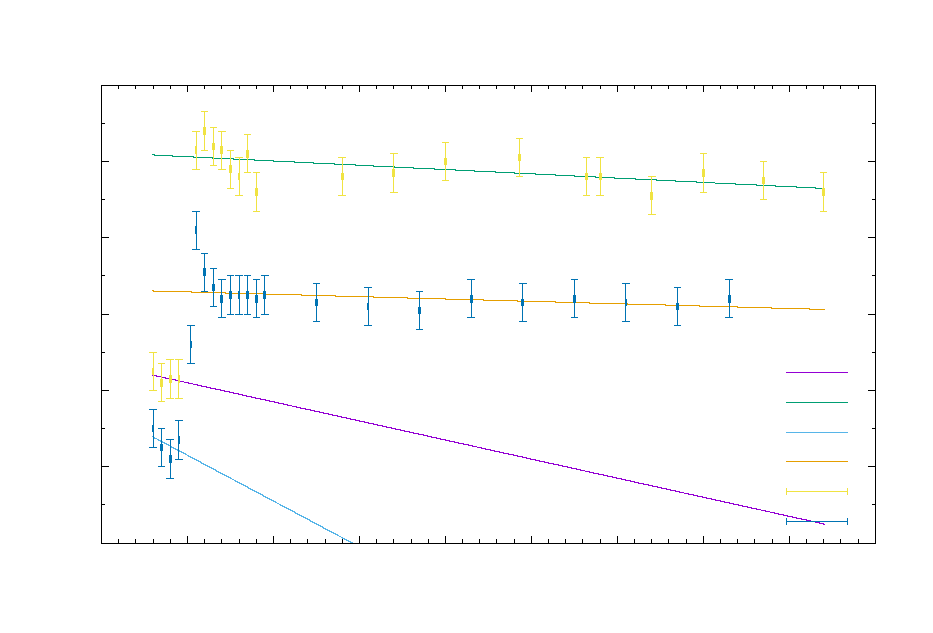
\includegraphics[width={432.00bp},height={288.00bp}]{tv2-plot}}%
    \gplfronttext
  \end{picture}%
\endgroup

		\caption{\centering Temperaturverlauf nach Eintauchen von Probekörpern ins Wasser}
		\label{fig:tvtwo-plot}
		\vspace{-1em}
	\end{figure}
	Als Endergebnis erhalten wir:
	\begin{align*}
		\begin{tabu}{lll}
			\toprule
			\text{Körper 1} & \text{Vorlauf:} & \theta = (\SI{-0.01000(1183)}{\celsius\per\second})t + \SI{26.200(162)}{\celsius} \\
			& \text{Nachlauf:} &  \theta = (\SI{-0.0022438(7261)}{\celsius\per\second})t + \SI{32.1258(1338)}{\celsius} \\
			\text{Körper 2} & \text{Vorlauf:} & \theta = (\SI{-0.02400(3274)}{\celsius\per\second})t + \SI{24.3000(4483)}{\celsius} \\
			& \text{Nachlauf:} &  \theta = (\SI{-0.001240(1241)}{\celsius\per\second})t + \SI{28.5819(1808)}{\celsius} \\
			\bottomrule
		\end{tabu}
	\end{align*}
	Gerundet:
	\begin{align*}
		\begin{tabu}{lll}
			\toprule
			\text{Körper 1} & \text{Vorlauf:} &  \theta = (\SI{-0.010(12)}{\celsius\per\second})t + \SI{26.20(17)}{\celsius} \\
			& \text{Nachlauf:} &   \theta = (\SI{-0.0022(8)}{\celsius\per\second})t + \SI{32.13(14)}{\celsius} \\
			\text{Körper 2} & \text{Vorlauf:} & \theta = (\SI{-0.02(4)}{\celsius\per\second})t + \SI{24.3(5)}{\celsius} \\
			& \text{Nachlauf:} &   \theta = (\SI{-0.0012(13)}{\celsius\per\second})t + \SI{28.58(19)}{\celsius} \\
			\bottomrule
		\end{tabu}
	\end{align*}
	Es ist hier zu bemerken, dass die Messpunkte große Abweichungen von der optimale Gerade haben. Außerdem ist die Gerade im Vorlaufbereich nicht in der richtige Richtung (nach unten statt nach oben). Die Daten sind also nicht besonders geeignet für diese Extrapolations\-verfahren. Die optimale Geraden wurden trotzdem dann auf Milimeterpapier im Bereich $[-50,50]$ gezeichnet, um die benötigte Werte zu finden. 

	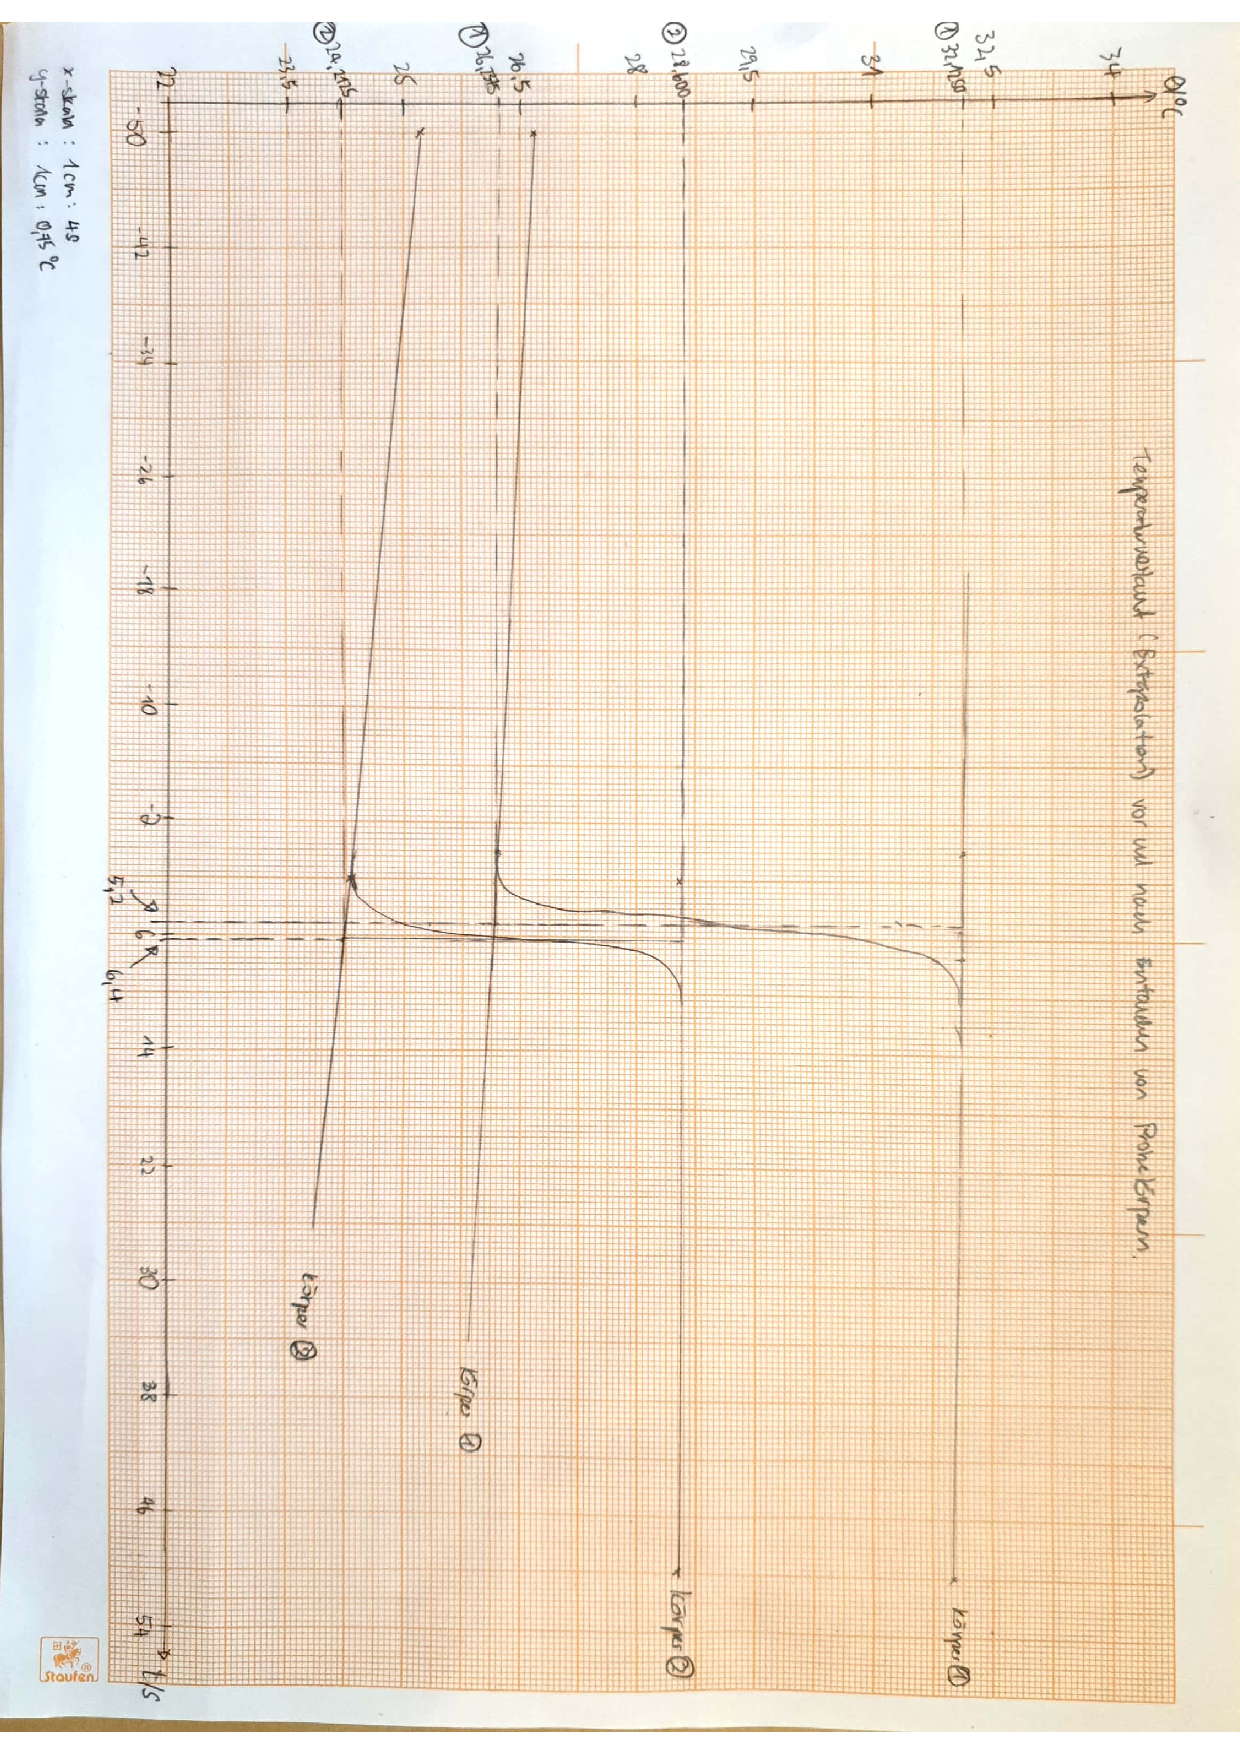
\includepdf{tv2-mm-paper.pdf}

	Wir erhalten als Ergebnis die Temperaturen:
	\begin{equation*}
		\begin{tabu}{llll}
			\toprule
			& \theta_a & \theta_e & t\\
			\midrule
			\text{Körper 1} & \SI{26.2375}{\celsius} & \SI{32.1250}{\celsius} & \SI{5.2}{\second}\\
			\text{Körper 2} & \SI{24.2125}{\celsius} & \SI{28.6000}{\celsius} & \SI{6.4}{\second}\\
			\bottomrule
		\end{tabu}
	\end{equation*}
	Wir berechnen nun die Min und Max anhand der Fehler bei der optimale Geraden aus \gnuplot{} am Zeitpunkt $t$ und erhalten:
	\begin{equation*}
		\begin{tabu}{llll}
			\toprule
			&& \theta_\text{max} & \theta_\text{min} \\
			\midrule
			\text{Körper 1} & \text{Anfang} & \SI{26.3804}{\celsius} & \SI{25.9156}{\celsius}\\
			 & \text{Ende} & \SI{32.26272}{\celsius} & \SI{31.9744}{\celsius}\\
			\text{Körper 2} & \text{Anfang} & \SI{24.928}{\celsius} & \SI{23.416}{\celsius}\\
			 & \text{Ende} & \SI{28.77064}{\celsius} & \SI{28.374}{\celsius}\\
			\bottomrule
		\end{tabu}
	\end{equation*}
	Also haben wir:
	\begin{equation*}
		\begin{tabu}{lll}
			\toprule
			& \theta_a & \theta_e \\
			\midrule
			\text{Körper 1} & \SI{26.15(23)}{\celsius} & \SI{32.12(15)}{\celsius} \\
			\text{Körper 2} & \SI{24.2(8)}{\celsius} & \SI{28.57(20)}{\celsius} \\
			\bottomrule
		\end{tabu}
	\end{equation*}
	$\theta_e$ ist in diesem Fall die Mischungstemperatur. 

	Aus der Anleitung gilt:
	\begin{align}
		c_s = \frac{c_w (m_w + m_w^*)(\Theta_m - \Theta_k)}{m_s(\Theta_s - \Theta_m)}
	\end{align}
	Wir berechnen zunächst den Wert und den entsprechenden Fehler von $m_w$ wie in Teilversuch 1:
	\begin{equation*}
		\begin{tabu}{llll}
			\toprule
			& M_\text{Wasser+Zyl} & M_\text{Zyl} & m_w \\
			\midrule
			\text{Körper 1} & \SI{1125.00(13)}{\gram} & \SI{307.57(3)}{\gram} & \SI{817.43(14)}{\gram} \\
			\text{Körper 2} & \SI{1095.80(13)}{\gram} & \SI{307.11(3)}{\gram} & \SI{788.69(14)}{\gram} \\
			\bottomrule
		\end{tabu}
	\end{equation*}
	\newpage
	\textbf{Körper 1 (Al)}

	Mit der Werten:
	\begin{center}
		\begin{tabular}{lll}
			\toprule
			Variable & Wert & Bedeutung \\
			\midrule
			$m_s$ & \SI{485.25(3)}{\gram} & Masse des Festkörpers \\
			$m_w$ & \SI{817.43(14)}{\gram} & Masse des Wassers \\
			$\Theta_m$ & \SI{32.12(15)}{\celsius} & Mischungstemperatur \\
			$\Theta_k$ & \SI{26.15(23)}{\celsius} & Temperatur des Wassers \\
			$\Theta_s$ & \SI{80.0(5)}{\celsius} & Temperatur des Festkörpers \\
			$m_w^*$ & \SI{80}{\gram} & Wasserwert des Kalorimeters \\
			$c_\text{w}$ & \SI{4.18}{\joule\per\gram\per\kelvin} & Spezifische Wärmekapazität des Wassers\\
			\bottomrule
		\end{tabular}
	\end{center}
	erhalten wir:
	\begin{align*}
		c_s &= \frac{(\SI{4.18}{\joule\per\gram\per\kelvin}) ((\SI{817.43}{\gram}) + (\SI{80}{\gram}))(\SI{32.12}{\celsius} - \SI{26.15}{\celsius})}{(\SI{485.25}{\gram})(\SI{80.0}{\celsius} - \SI{32.12}{\celsius})} \\
		&= \SI{0.9639}{\joule\per\gram\per\kelvin} \sigfig{4}
	\end{align*}
	Mittels der Min-Max-Methode erhalten wir:
	\begin{center}
		\begin{tabular}{lll}
			\toprule
			Min & Max & Wert \\
			\midrule
			\SI{0.8901}{\joule\per\gram\per\kelvin} & \SI{1.0398}{\joule\per\gram\per\kelvin} & \SI{0.96(8)}{\joule\per\gram\per\kelvin} \\
			\bottomrule
		\end{tabular}
	\end{center}
	\textbf{Körper 2 (Pb)}

	Mit der Werten:
	\begin{center}
		\begin{tabular}{lll}
			\toprule
			Variable & Wert & Bedeutung \\
			\midrule
			$m_s$ & \SI{1945.80(13)}{\gram} & Masse des Festkörpers \\
			$m_w$ & \SI{788.69(14)}{\gram} & Masse des Wassers \\
			$\Theta_m$ & \SI{28.57(20)}{\celsius} & Mischungstemperatur \\
			$\Theta_k$ & \SI{24.2(8)}{\celsius} & Temperatur des Wassers \\
			$\Theta_s$ & \SI{77.7(5)}{\celsius} & Temperatur des Festkörpers \\
			$m_w^*$ & \SI{80}{\gram} & Wasserwert des Kalorimeters \\
			$c_\text{w}$ & \SI{4.18}{\joule\per\gram\per\kelvin} & Spezifische Wärmekapazität des Wassers\\
			\bottomrule
		\end{tabular}
	\end{center}
	erhalten wir:
	\begin{align*}
		c_s &= \frac{(\SI{4.18}{\joule\per\gram\per\kelvin}) (\SI{788.69}{\gram} + \SI{80}{\gram})(\SI{28.57}{\celsius} - \SI{24.2}{\celsius})}{(\SI{1945.80}{\gram})(\SI{77.7}{\celsius} - \SI{28.57}{\celsius})} \\
		&= \SI{0.1660}{\joule\per\gram\per\kelvin} \sigfig{4}
	\end{align*}
	Mittels der Min-Max-Methode erhalten wir:
	\begin{center}
		\begin{tabular}{lll}
			\toprule
			Min & Max & Wert \\
			\midrule
			\SI{0.12618}{\joule\per\gram\per\kelvin} & \SI{0.20697}{\joule\per\gram\per\kelvin} & \SI{0.17(5)}{\joule\per\gram\per\kelvin} \\
			\bottomrule
		\end{tabular}
	\end{center}
	\newpage
	Zusammengefasst haben wir mit $C_m = C_s \times M_R$ ($M_R$ molare Masse):
	\begin{equation*}
		\begin{tabu}{lll}
			\toprule
			& C_s & C_m \\
			\midrule
			\text{Körper 1 (Al)} & \SI{0.96(8)}{\joule\per\gram\per\kelvin} & \SI{25.9(22)}{\joule\per\mole\per\kelvin} \\
			\text{Körper 2 (Pb)} & \SI{0.17(5)}{\joule\per\gram\per\kelvin} & \SI{35(11)}{\joule\per\mole\per\kelvin} \\
			\bottomrule
		\end{tabu}
	\end{equation*}
	Nach Regel von Dulong und Petit gilt:
	\begin{equation}
		C_\text{v}^\text{m} = 3R = 3 (\SI{8.31}{\joule\per\mole\per\kelvin}) = \SI{24.93}{\joule\per\mole\per\kelvin}
	\end{equation}
	Dieser Literaturwert liegt in dem Fehlerintervall von beiden experimental bestimmten Werten, also stimmen die Ergebnisse mit dem Literaturwert überein.

